\chapter{Detektoren in der Teilchenphysik}
Was wir wissen wollen:
\begin{itemize}
	\item Transversalimpuls $p_\text{T}$
	\item Polarwinkel $\phi$
	\item (Pseudo)rapidität (also Azimuthwinkel) $\eta$
	\item Energie
	\item Teilchenart.
\end{itemize}

\section{Die Blasenkammer}
Das Prinzip der Blasenkammer ist einfach:
Die Flüssigkeit (z.B. H2) im Unterdruck beginnt an Verunreinigungen und Ionisationskeimen zu sieden.
Diese Bläschen werden fotografiert.
Das ist zum einen sehr ungenau und zum anderen können wir so keine Aussagen über die Teilchenart machen.

\section{Nachweismethoden für Teilchen}
\begin{figure}
	\centering
	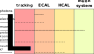
\includegraphics[width=.7\textwidth]{./img/detectorsystem.pdf}
	\caption{Verschiedene Teilchen können durch die Ebenen unterschieden werden.}
	\label{fig:detectionmethods}
\end{figure}
Um verschiedene Teilchenarten zu unterscheiden, ist ein Detektor durch mehrere Ebenen aufgebaut (siehe \autoref{fig:detectionmethods}).

\textbf{Die tracking layer} sorgt für eine Richtungsbestimmung.

\textbf{Das elektromagnetische Kalorimeter} bestimmt die Energie von Teilchen die im Wesentlichen über die elektromagnetische Kraft wechselwirken.

\textbf{Im hadronischen Kalorimeter} lassen sich Teilchen nachweisen, die überwiegend der starken Wechselwirkung unterliegen.
Da hadronische Teilchen szintillierendes Material fast ungehindert durchdringen ist der Nachweis über das em-Kalorimeter nicht gewährleistet.

\textbf{Im Myon-System} werden die hochenergetischen Myonen nachgewiesen, da sie für einen Nachweis im em-Kalorimeter zu hochenergetisch sind.

Der Teilchennachweis erfolgt über
\begin{itemize}
	\item Ionisation des Detektormaterials
	\item Bremsstrahlung/Paarbildung in em-Feldern im Detektormaterial und
	\item Kernwechselwirkungen mit dem Detektormaterial.
\end{itemize}

\section{Spurdetektoren}
\subsection{Gasgefüllte Spurdetektoren}
Hereinkommende geladene Teilchen ionisieren das Gas im Detektor und hinterlassen dabei eine Spur.
Ionisierte Ladungen bewegen sich entlang eines elektrischen Feldes zur Kathode bzw. Anode.
Je nach dem, in welchem Bereich der Kennlinie man sich bewegt unterscheidet man zwischen
\begin{itemize}
	\item \textbf{Proportionalkammern}, die im linearen Bereich der Kennlinie betrieben werden. Dabei ist die Anzahl der Ionenpaare proportional zur Primärionisation.
	\item \textbf{Geiger-Müller-Zählrohren}, die in der Plateauregion betrieben werden und damit keine Proportionalität zur Primärionisation aufweisen.
\end{itemize}
\subsubsection{Vieldrahtproportionalkammern}
bestehen aus vielen parallel angeordneten Anodendrähten. Es lässt sich somit eine 1D-Ortsinformation bestimmen und da sie im Proportionalbetrieb sind, auch die Teilchenenergie in einem bestimmten Bereich.

\subsubsection{Driftkammern}
lösen das Problem der limitierten Ortsauflösung durch den Drahtabstand bei MWPCs. Die Ionen brauchen eine bestimmte Zeit, um zum Anodendraht zu wandern. Diese Zeit $\Delta t$ kann dazu verwenden werden, um eine Ortsinformation zu erhalten nach
\begin{equation*}
	x' = x_0 + \frac{e}{2m}\mvec{E}(\mvec{r})\Delta t.
\end{equation*}
In Zeitprojektionskammern kann man so sogar eine 3D-Ortsbestimmung machen: 2D über die Projektion auf die Anoden, 1D über die Driftzeitinformation.

\subsection{Siliziumdetektoren}
Eleganter, aber kostenaufwändiger lässt sich das mit Siliziumdetektoren in Sperrrichtung lösen, wie am CMS der Fall.
Dabei beträgt die Impulsauflösung ca. 0.5\%.
Die Impulsbestimmung folgt aus dem assoziierten Zyklotronradius der Teilchenspur über
\begin{equation*}
	p[\si{\GeV}] = 0.3\cdot r[\si{\meter}] \cdot B[\si{\tesla}].
\end{equation*}

\section{Kalorimeter}
Das Kalorimeter schließt sich an die Spurdetektoren an und misst die Energie aller erzeugten und nachweisbaren Teilchen.
Dabei werden verschiedene Phänomene ausgenutzt
\begin{itemize}
	\item Energieverlust durch Ionisation
	\item Sammlung von Szintillationslicht
	\item Elektromagnetische und hadronische Schauerbildung.
\end{itemize}
Das Kalorimeter muss dabei dick genug sein, um die Teilchenschauer vollständig im aktiven Material zu stoppen, andernfalls gehen Informationen verloren.
Das Szintillationslicht wird dann durch Photomultiplier ausgelesen.

\subsection{Elektromagnetische Schauer}
Sind Kaskaden aus Photonen und Elektron-Positron-Paaren.
Grundlage der Schauerbildung ist dabei die Bremsstrahlung und Paarerzeugung.
Die \textbf{Strahlungslänge} gibt dabei eine Längenskala für den Teilchenschauen an.
Er ist definiert durch
\begin{equation*}
	-\frac{\text{d}E}{\text{d}X} = \frac{E}{X_0}
\end{equation*}
und ist abhängig vom Material.

\subsection{Hadronische Schauer}
Sind Kaskaden, die durch ein Hadron ausgelöst werden.
Grundlage ist hier die starke Wechselwirkung (Hadronisierung, Zerfall).
Da neutrale Hadronen in zwei Photonen zerfallen können, lösen hadronische Schauer auch elektromagnetische Schauer aus.
